\documentclass[10pt,a4paper]{article}
\usepackage[utf8]{inputenc}
\usepackage[T1]{fontenc}
\usepackage{amsmath}
\usepackage{amssymb}
\usepackage{graphicx}
\usepackage[english,russian]{babel} 
\usepackage{fontspec} 
\setmainfont{Times New Roman}
\title{Отчет по лабораторной работе №2}
\author{Ивлев А.Е Б19-511}
\usepackage{graphicx}
\graphicspath{{./Graphics/}}
\DeclareGraphicsExtensions{.pdf,.png,.jpg,.eps}
\begin{document}
	\maketitle
	
	\begin{figure}[h]
		\centering
		{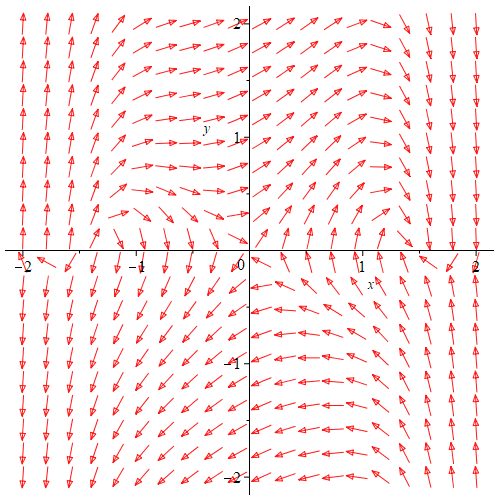
\includegraphics[scale=0.3]{Lab2 phase portrait a=-1, b=0.5}}
		{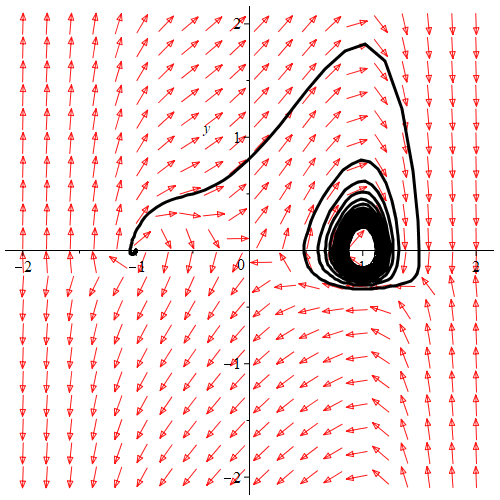
\includegraphics[scale=0.3]{Lab2 phase portrait a=-1, b=1}}
		\caption{Фазовые портреты при $a = -1$, $b = 0.5$; $a = -1$, $b = 1$}
		\label{image/1}
	\end{figure}

	Исходная динамическая система:

	\begin{equation}
		\label{math/1}
		\begin{cases}
			\dot{x} = y, \\
			\dot{y} = b(1-x^{5})y - a x - b x^3.
		\end{cases}
	\end{equation}

	Для начала воспользуемся критерием Бендиксона.
	\begin{equation}
		\label{math/2}
		\begin{cases}
			\ \frac{\partial f(x, y)}{\partial x} = 0 \\
			\ \frac{\partial g(x, y)}{\partial y} = b(1 - x^5).
		\end{cases}
	\end{equation}
	
	Здесь $f(x,y)$ и $g(x,y)$ - правые части исходной системы. Сумма $f_x(x,y) + g_y(x,y)$ меняет свой знак при пересечении прямой $x = 1$. Примем параметр $b$ за положительную величину. Тогда справа от $x = 1$ выражение $f_x + g_y > 0$, а слева $f_x + g_y < 0$. В данном случае согласно критерию Бендиксона замкнутая траектория не может не пересекать прямую $x = 1$.
	
	Для получения большей информации воспользуемся теорией индексов. Найдем все точки покоя системы. Приравнивая к нулю правые части, находим 3 точки покоя: $(0;0)$, $(-\sqrt{-a/b}; 0)$ и $(\sqrt{-a/b}; 0)$.
	
	Примем параметр $a = -1$.
	
	Находя собственные значения для матриц Якоби в точках покоя получаем, что $(0;0)$ - седло ($I_0 = -1$) и  $(-\sqrt{1/b}; 0)$ тоже седло ($I_1 = -1$) при любых положительных значениях параметра $b$.
	
	Точка $(\sqrt{1/b}; 0)$ является седлом при $b \in (0; ~0,79)$, $I_2 = -1$. В этом случае замкнутая траектория нигде не возможна. При $b \in (~0,79; ~0,81)$ устойчивый узел, $I_2 = 1$. Возможна замкнутая траектория, охватывающая эту точку и пересекающая прямую $x = 1$. В случае $b \in (~143,94; \infty)$ узел будет неустойчивым. При $b \in (~0,81; ~143,94)$ собственные значения станут комплексными. Точка покоя станет фокусом, $I_2 = 1$, замкнутая траектория возможна.
	
\end{document}